%!TEX TS-program = /usr/texbin/pdflatex
%!GEDIT texbin = /usr/local/texlive/current/bin/x86_64-linux/pdflatex
%
%	''Becker-Vorlage'' style LaTeX template

% 	This template is  MIT licensed, authors:
%   Jan Betzing <jan.betzing@ercis.uni-muenster.de> *corresponding author
%	Dominik Lekse <dominik@lekse.de>
%
% 	Basic file to demonstrate the usage of this LaTeX template.
% 	You can build your own paper/thesis on top of this file.
% 	Simply adjust the document class and all metadata and start working.
%
\documentclass[
  language=german, % set to english or german
  type=bachelor% set to bachelor, master or seminar
]{isthesis}

% Graphics rendering using TikZ
% See: https://en.wikibooks.org/wiki/LaTeX/PGF/TikZ
\usepackage{tikz}
% Include required TikZ libraries here, some exemplary libraries are pre-included
\usetikzlibrary{calc}
\usetikzlibrary{matrix}
\usetikzlibrary{positioning}
\usetikzlibrary{shapes.geometric}

% Import acronyms
\input{lib/acronyms}

% Import symbols
\input{lib/symbols}

% Document meta information
\isthesis{title={Methode und Sprache für die Analyse von Unternehmensdaten und Entwicklung einer Webanwendung für deren konzeptionelle Umsetzung \newline \newline Methode und Sprache für die Analyse von Unternehmensdaten innerhalb von DataRocket und Implementierung des strukturellen Aspekts einer entsprechenden Berichtskomponente},
  author={Max Leonard Inden},
  author-email={max.inden@uni-muenster.de},
  author-phone={+49 178 1493411}, % Use international numbers format
  author-matriculation={409098},
  author-address={Biemsmaar 4c},
  author-zip={53343},
  author-city={Wachtberg},
  principal-supervisor={Prof.\ Dr.\ Dr.\ h.c. Dr.\ h.c. J\"org Becker}, % This has to be a professor
  associate-supervisor={Dr.\ Stefan Fleischer}, % This is your main supervisor, i.e., a post doc or PhD student
  tutor-supervisor={}, % If required, define an additional supervisor resp. tutor here
  group={Lehrstuhl für Wirtschaftsinformatik und Informationsmanagement},
  group-institute={Westfälische Wilhelms-Universität, M\"unster},
  associate-group={innoscale AG}, % When the thesis is done in cooperation with another chair, add it here
  %associate-group-institute={innoscale AG}, % add cooperating institute or university here
  seminar={Scientific Writing for Beginners}, % The title of your seminar
  submission-date={}, % !!! In  isthesis.cls ändern
  %primary-logo={}, % Uses the WWU logo by default
  %primary-logo-height={}, % Uses 16mm as default height
  secondary-logo={lib/assets/innoscale-logo}, % Logo of the secondary institution (cooperating chair/university), USES Faculty logo by default
  %secondary-logo-height={} % Uses 16mm as default height
}
\begin{document}
% Title page
\maketitle

% Quote
% You can put an optional quote page in front of your content
%\quotepage[author={Arthur C. Clarke}]{
%  Any sufficiently advanced technology is indistinguishable from magic.
%}

% Table of contents
\tableofcontents

% List of figures (if you have figures)
%\listoffigures

% List of tables (if you have tables)
%\listoftables

% List of listings (if you have listings)
%\lstlistoflistings{}

% List of abbreviations (if you use acronyms)
\listofabbreviations{}
% List of symbols (if you use symbols)
%\listofsymbols{}

% Abstract
%
% Comment out this part, if you don't require an abstract
%\begin{abstract}
%  \input{content/abstract}
%\end{abstract}

% Content
\begin{content}
% ################################################################################
% \chapter{Bachelorarbeit Proposal}


\section{Ziele}
\begin{itemize}
  \item Konzeption einer \textbf{Datenstruktur-Metasprache} angelehnt an
    \textit{H2 for reporting}, welche sich nach den Ansprüchen 
    \begin{itemize}
      \item Abbildung komplexer hierarchischer Datenstrukturen
      \item Beschreibung ihrer modularen Beziehungen sowie
      \item Spezifikation von Kennzahlen und deren Berechnung auf Basis
        verschiedener Ebenen der hierarchischen Datenstruktur
    \end{itemize}
    von innoscale richtet.
  \item Entwicklung einer \textbf{Web-Applikation} zur Anwendung der
    Datenstruktur-Metasprache welche
    \begin{itemize}
      \item die Spezifikation einer Datenstruktur zum Aufbau eines \acrshort{DWH} und
      \item die Spezifikation von Berichten aus einer spezifizierten
        \acrshort{DWH} Datenstruktur
    \end{itemize}
    ermöglicht. Diese Applikation soll für den Benutzer grafisch ansprechend
    und leicht zu bedienen sein.
\end{itemize}


\section{Vorgehen}
\begin{enumerate}
  \item Vergleich verschiedener Sprachdialekte (\textit{H2 for reporting} etc.)
  \item Sichtung weiterer Literaturquellen zum Thema Metadatenmanagement
  \item Erkunden des H2 Toolsets im Zusammenhang mit \textit{H2 for
    reporting}
  \item Konzeption der innoscale spezifischen Datenstruktur-Metasprache in
    enger Absprache mit innoscale
  \item Konzeption der Web-Applikation
  \item Entwicklung der Web-Applikation
  \item Ausblick: Integration der entwickelten Lösung in DataRocket
    (konzeptionell)
\end{enumerate}


% ################################################################################



% ################################################################################
\chapter{Einleitung}
% ################################################################################

  \section{Vorstellung innoscale AG}
  Die \textit{innoscale AG} ist ein im Jahre 2013 gegründetes Unternehmen aus
  Berlin.  Spezialisiert auf das Stammdatenmanagement ist es sowohl beratend
  als auch mit einem eigenen Produkt zur Verbesserung der Datenqualität namens
  \textit{DataRocket}\footnote{Siehe Abschnitt: Vorstellug
  DataRocket~\ref{sec:Vorstellung-DataRocket}} tätig. Im Rahmen der
  Datenqualitätsverbesserung ist es nötig die Qualität von zuvor strukturierten
  Daten anhand von Kennzahlen auszuwerten und zu visualieren.

\section{Status quo und Problemstellung}
\begin{itemize}
  \item Die Daten sind vorhanden
  \item Auswertung bisher nur mit dem nötigen EDV-Wissen möglich
  \item Für technischen Laien sind die Daten unbrauchbar
  \item Daten enthalten wirtschaftlich relevante Fakten
  \item Daten sind komplex
\end{itemize}

\section{Ziel}
\begin{itemize}
  \item Spezifikation einer Datenanalysepraktik zugeschnitten auf das
    Unternehmen \textit{innoscale AG}
  \begin{itemize}
    \item Leicht verständlich
    \item Modellierung von Datenstrukturen, Kennzahlen und die Kombination der
      beiden als Fakten/Tabelle
    \item Datenstruktur generiert aus einem SQL-Schema
    \item Kennzahlen: Modellierung aller gängigen arithmentischen Operationen
    \item Fakten/Tabelle: mit Zeilen und Spalten aus Datenstruktur und Kennzahl 
  \end{itemize}
\item DataRocket-Komponente zur Konzeption von Datenauswertungen
  \begin{itemize}
    \item Spezifikation von Datenstrukturen, Kennzahlen und Tabellen
    \item Leicht verständlich und grafisch ansprechend
    \item Benutzbar für technischen Laien
  \end{itemize}
\end{itemize}




% ################################################################################
  \chapter{Methode und Sprache zur Analyse von Unternehmensdaten}
% ################################################################################

  \section{Existierende Methoden und Sprachen zur Analyse von Unternehmensdaten}
  \begin{itemize}
    \item H2ForReporting
    \item Cognos
    \item Palos
  \end{itemize}

  \section{Beispielszenario}
  Für den weiteren Verlauf dieser Arbeit wird ein Beispielszenario vorgestellt. Im
  Fokus steht eine fiktive Firma namens SmartSell. SmartSell setzt seine
  Produkte sowohl klassisch über ihr lokales Geschäft, als auch über einen
  eigenen Online-Shop ab.

  Beispiel Dimensionen
  \begin{itemize}
    \item Absatzkanal
    \item Zeit
    \item Produkt
    \item Ort
    \item Kunde
    \item Personal
    \item Lieferant
    \item Wertansatz (Soll, Ist, Plan)
  \end{itemize}

  \section{Rahmenbedingungen und Annahmen}
  \begin{itemize}
    \item Input Daten voll normalisiert
    \item Star-Schema denormalisiert
    \item Snow-Schema normalisiert
  \end{itemize}

  \section{innoscale DataFurnace-Sprache und -Methode}
  \texthl{Ein Subset von H2ForReporting? F\"ur DQM statt f\"ur Business Intelligence?}

  \subsection{Sprache}
  \begin{figure}[caption={Relationship of students and theses}, label={fig:img01}]
    \resizebox{\columnwidth}{!}{% Graphic for TeX using PGF
% Title: /home/indenml/ownCloud/wwu_wi/s6/bachelorarbeit/graphics/object-erm.dia
% Creator: Dia v0.97.3
% CreationDate: Thu Jul 21 15:40:48 2016
% For: indenml
% \usepackage{tikz}
% The following commands are not supported in PSTricks at present
% We define them conditionally, so when they are implemented,
% this pgf file will use them.
\ifx\du\undefined
  \newlength{\du}
\fi
\setlength{\du}{15\unitlength}
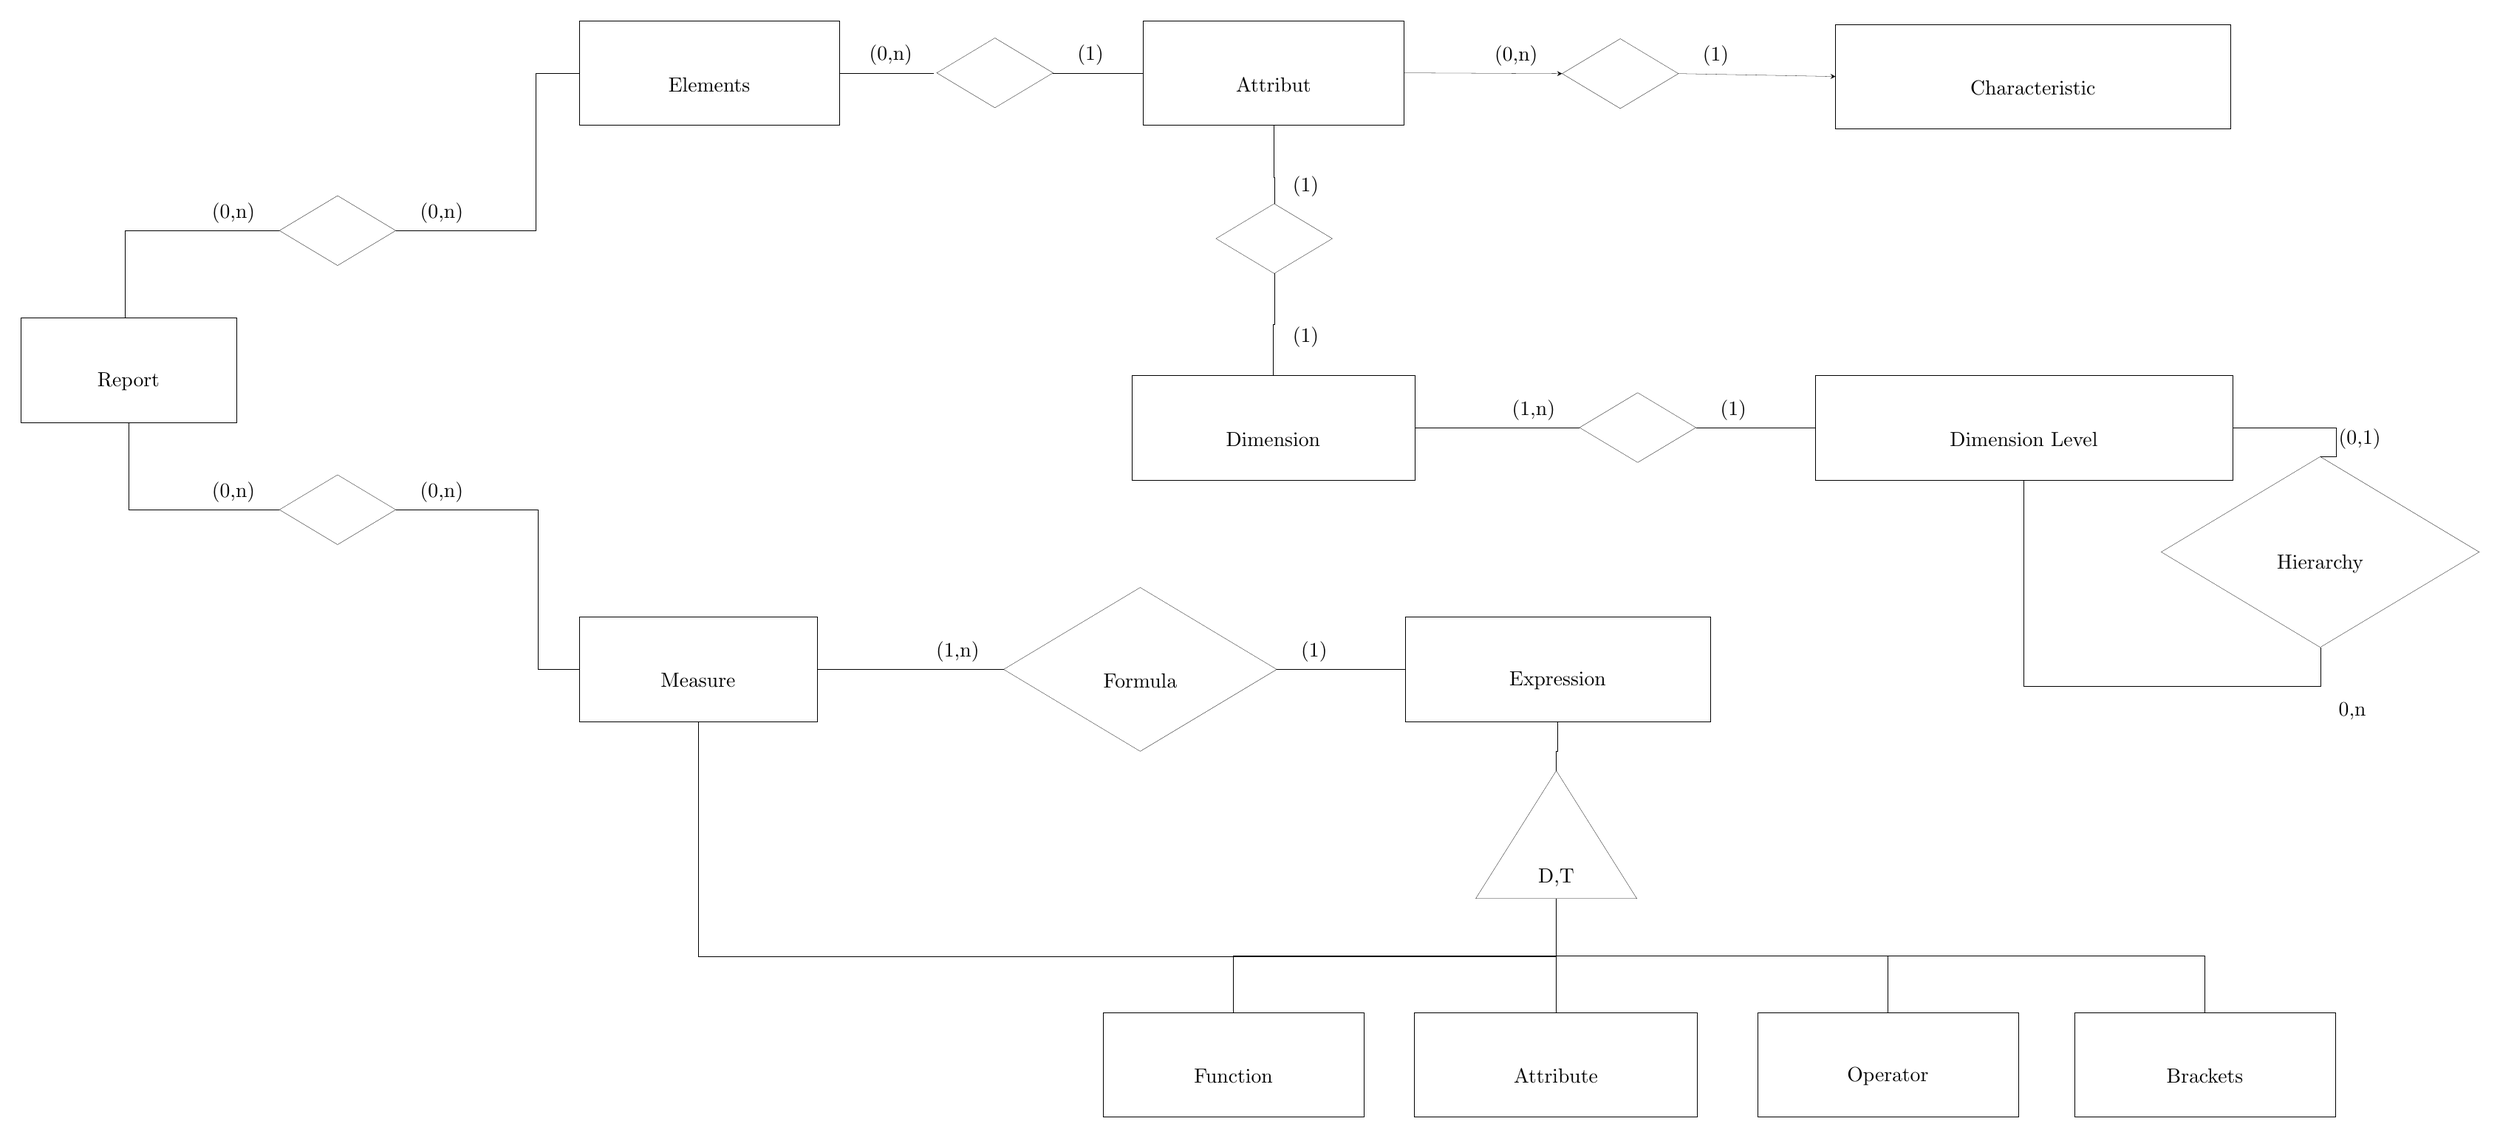
\begin{tikzpicture}
\pgftransformxscale{1.000000}
\pgftransformyscale{-1.000000}
\definecolor{dialinecolor}{rgb}{0.000000, 0.000000, 0.000000}
\pgfsetstrokecolor{dialinecolor}
\definecolor{dialinecolor}{rgb}{1.000000, 1.000000, 1.000000}
\pgfsetfillcolor{dialinecolor}
\definecolor{dialinecolor}{rgb}{1.000000, 1.000000, 1.000000}
\pgfsetfillcolor{dialinecolor}
\fill (24.900000\du,18.850000\du)--(24.900000\du,20.650000\du)--(29.765000\du,20.650000\du)--(29.765000\du,18.850000\du)--cycle;
\pgfsetlinewidth{0.100000\du}
\pgfsetdash{}{0pt}
\pgfsetmiterjoin
\definecolor{dialinecolor}{rgb}{0.000000, 0.000000, 0.000000}
\pgfsetstrokecolor{dialinecolor}
\draw (24.900000\du,18.850000\du)--(24.900000\du,20.650000\du)--(29.765000\du,20.650000\du)--(29.765000\du,18.850000\du)--cycle;
% setfont left to latex
\definecolor{dialinecolor}{rgb}{0.000000, 0.000000, 0.000000}
\pgfsetstrokecolor{dialinecolor}
\node at (27.332500\du,19.950000\du){Dimension};
\definecolor{dialinecolor}{rgb}{1.000000, 1.000000, 1.000000}
\pgfsetfillcolor{dialinecolor}
\fill (36.650000\du,18.850000\du)--(36.650000\du,20.650000\du)--(43.825000\du,20.650000\du)--(43.825000\du,18.850000\du)--cycle;
\pgfsetlinewidth{0.100000\du}
\pgfsetdash{}{0pt}
\pgfsetmiterjoin
\definecolor{dialinecolor}{rgb}{0.000000, 0.000000, 0.000000}
\pgfsetstrokecolor{dialinecolor}
\draw (36.650000\du,18.850000\du)--(36.650000\du,20.650000\du)--(43.825000\du,20.650000\du)--(43.825000\du,18.850000\du)--cycle;
% setfont left to latex
\definecolor{dialinecolor}{rgb}{0.000000, 0.000000, 0.000000}
\pgfsetstrokecolor{dialinecolor}
\node at (40.237500\du,19.950000\du){Dimension Level};
\definecolor{dialinecolor}{rgb}{1.000000, 1.000000, 1.000000}
\pgfsetfillcolor{dialinecolor}
\fill (15.400000\du,12.750000\du)--(15.400000\du,14.550000\du)--(19.880000\du,14.550000\du)--(19.880000\du,12.750000\du)--cycle;
\pgfsetlinewidth{0.100000\du}
\pgfsetdash{}{0pt}
\pgfsetmiterjoin
\definecolor{dialinecolor}{rgb}{0.000000, 0.000000, 0.000000}
\pgfsetstrokecolor{dialinecolor}
\draw (15.400000\du,12.750000\du)--(15.400000\du,14.550000\du)--(19.880000\du,14.550000\du)--(19.880000\du,12.750000\du)--cycle;
% setfont left to latex
\definecolor{dialinecolor}{rgb}{0.000000, 0.000000, 0.000000}
\pgfsetstrokecolor{dialinecolor}
\node at (17.640000\du,13.850000\du){Elements};
\definecolor{dialinecolor}{rgb}{1.000000, 1.000000, 1.000000}
\pgfsetfillcolor{dialinecolor}
\fill (25.100000\du,12.750000\du)--(25.100000\du,14.550000\du)--(29.580000\du,14.550000\du)--(29.580000\du,12.750000\du)--cycle;
\pgfsetlinewidth{0.100000\du}
\pgfsetdash{}{0pt}
\pgfsetmiterjoin
\definecolor{dialinecolor}{rgb}{0.000000, 0.000000, 0.000000}
\pgfsetstrokecolor{dialinecolor}
\draw (25.100000\du,12.750000\du)--(25.100000\du,14.550000\du)--(29.580000\du,14.550000\du)--(29.580000\du,12.750000\du)--cycle;
% setfont left to latex
\definecolor{dialinecolor}{rgb}{0.000000, 0.000000, 0.000000}
\pgfsetstrokecolor{dialinecolor}
\node at (27.340000\du,13.850000\du){Attribut};
\definecolor{dialinecolor}{rgb}{1.000000, 1.000000, 1.000000}
\pgfsetfillcolor{dialinecolor}
\fill (42.600000\du,21.889500\du)--(45.332500\du,20.250000\du)--(48.065000\du,21.889500\du)--(45.332500\du,23.529000\du)--cycle;
\pgfsetlinewidth{0.100000\du}
\pgfsetdash{}{0pt}
\pgfsetmiterjoin
\definecolor{dialinecolor}{rgb}{0.000000, 0.000000, 0.000000}
\pgfsetstrokecolor{dialinecolor}
\draw (42.600000\du,21.889500\du)--(45.332500\du,20.250000\du)--(48.065000\du,21.889500\du)--(45.332500\du,23.529000\du)--cycle;
% setfont left to latex
\definecolor{dialinecolor}{rgb}{0.000000, 0.000000, 0.000000}
\pgfsetstrokecolor{dialinecolor}
\node[anchor=west] at (45.532500\du,19.950000\du){(0,1)};
\definecolor{dialinecolor}{rgb}{0.000000, 0.000000, 0.000000}
\pgfsetstrokecolor{dialinecolor}
\node[anchor=west] at (45.532500\du,24.629000\du){0,n};
\definecolor{dialinecolor}{rgb}{0.000000, 0.000000, 0.000000}
\pgfsetstrokecolor{dialinecolor}
\node at (45.332500\du,22.089500\du){Hierarchy};
\pgfsetlinewidth{0.100000\du}
\pgfsetdash{}{0pt}
\pgfsetmiterjoin
\pgfsetbuttcap
\definecolor{dialinecolor}{rgb}{0.000000, 0.000000, 0.000000}
\pgfsetstrokecolor{dialinecolor}
\draw (40.237500\du,20.650000\du)--(40.237500\du,24.200000\du)--(45.332500\du,24.200000\du)--(45.332500\du,23.529000\du);
\pgfsetlinewidth{0.100000\du}
\pgfsetdash{}{0pt}
\pgfsetmiterjoin
\pgfsetbuttcap
\definecolor{dialinecolor}{rgb}{0.000000, 0.000000, 0.000000}
\pgfsetstrokecolor{dialinecolor}
\draw (43.825000\du,19.750000\du)--(45.600000\du,19.750000\du)--(45.600000\du,20.250000\du)--(45.332500\du,20.250000\du);
\definecolor{dialinecolor}{rgb}{1.000000, 1.000000, 1.000000}
\pgfsetfillcolor{dialinecolor}
\fill (32.600000\du,19.750000\du)--(33.600000\du,19.150000\du)--(34.600000\du,19.750000\du)--(33.600000\du,20.350000\du)--cycle;
\pgfsetlinewidth{0.100000\du}
\pgfsetdash{}{0pt}
\pgfsetmiterjoin
\definecolor{dialinecolor}{rgb}{0.000000, 0.000000, 0.000000}
\pgfsetstrokecolor{dialinecolor}
\draw (32.600000\du,19.750000\du)--(33.600000\du,19.150000\du)--(34.600000\du,19.750000\du)--(33.600000\du,20.350000\du)--cycle;
% setfont left to latex
\definecolor{dialinecolor}{rgb}{0.000000, 0.000000, 0.000000}
\pgfsetstrokecolor{dialinecolor}
\node[anchor=east] at (32.300000\du,19.450000\du){(1,n) };
\definecolor{dialinecolor}{rgb}{0.000000, 0.000000, 0.000000}
\pgfsetstrokecolor{dialinecolor}
\node[anchor=west] at (34.900000\du,19.450000\du){(1) };
\definecolor{dialinecolor}{rgb}{0.000000, 0.000000, 0.000000}
\pgfsetstrokecolor{dialinecolor}
\node at (33.600000\du,19.950000\du){};
\pgfsetlinewidth{0.100000\du}
\pgfsetdash{}{0pt}
\pgfsetmiterjoin
\pgfsetbuttcap
\definecolor{dialinecolor}{rgb}{0.000000, 0.000000, 0.000000}
\pgfsetstrokecolor{dialinecolor}
\draw (29.765000\du,19.750000\du)--(29.815000\du,19.750000\du)--(32.550000\du,19.750000\du)--(32.600000\du,19.750000\du);
\pgfsetlinewidth{0.100000\du}
\pgfsetdash{}{0pt}
\pgfsetmiterjoin
\pgfsetbuttcap
\definecolor{dialinecolor}{rgb}{0.000000, 0.000000, 0.000000}
\pgfsetstrokecolor{dialinecolor}
\draw (34.600000\du,19.750000\du)--(34.650000\du,19.750000\du)--(36.600000\du,19.750000\du)--(36.650000\du,19.750000\du);
\definecolor{dialinecolor}{rgb}{1.000000, 1.000000, 1.000000}
\pgfsetfillcolor{dialinecolor}
\fill (21.550000\du,13.650000\du)--(22.550000\du,13.050000\du)--(23.550000\du,13.650000\du)--(22.550000\du,14.250000\du)--cycle;
\pgfsetlinewidth{0.100000\du}
\pgfsetdash{}{0pt}
\pgfsetmiterjoin
\definecolor{dialinecolor}{rgb}{0.000000, 0.000000, 0.000000}
\pgfsetstrokecolor{dialinecolor}
\draw (21.550000\du,13.650000\du)--(22.550000\du,13.050000\du)--(23.550000\du,13.650000\du)--(22.550000\du,14.250000\du)--cycle;
% setfont left to latex
\definecolor{dialinecolor}{rgb}{0.000000, 0.000000, 0.000000}
\pgfsetstrokecolor{dialinecolor}
\node[anchor=east] at (21.250000\du,13.350000\du){(0,n)};
\definecolor{dialinecolor}{rgb}{0.000000, 0.000000, 0.000000}
\pgfsetstrokecolor{dialinecolor}
\node[anchor=west] at (23.850000\du,13.350000\du){(1)};
\definecolor{dialinecolor}{rgb}{0.000000, 0.000000, 0.000000}
\pgfsetstrokecolor{dialinecolor}
\node at (22.550000\du,13.850000\du){};
\pgfsetlinewidth{0.100000\du}
\pgfsetdash{}{0pt}
\pgfsetmiterjoin
\pgfsetbuttcap
\definecolor{dialinecolor}{rgb}{0.000000, 0.000000, 0.000000}
\pgfsetstrokecolor{dialinecolor}
\draw (19.880000\du,13.650000\du)--(19.930000\du,13.650000\du)--(21.450177\du,13.650000\du)--(21.500177\du,13.650000\du);
\pgfsetlinewidth{0.100000\du}
\pgfsetdash{}{0pt}
\pgfsetmiterjoin
\pgfsetbuttcap
\definecolor{dialinecolor}{rgb}{0.000000, 0.000000, 0.000000}
\pgfsetstrokecolor{dialinecolor}
\draw (23.550000\du,13.650000\du)--(23.600000\du,13.650000\du)--(25.050000\du,13.650000\du)--(25.100000\du,13.650000\du);
\pgfsetlinewidth{0.100000\du}
\pgfsetdash{}{0pt}
\pgfsetmiterjoin
\pgfsetbuttcap
\definecolor{dialinecolor}{rgb}{0.000000, 0.000000, 0.000000}
\pgfsetstrokecolor{dialinecolor}
\draw (27.340000\du,14.550000\du)--(27.340000\du,15.450000\du)--(27.350000\du,15.450000\du)--(27.350000\du,15.900000\du);
\definecolor{dialinecolor}{rgb}{1.000000, 1.000000, 1.000000}
\pgfsetfillcolor{dialinecolor}
\fill (26.350000\du,16.500000\du)--(27.350000\du,15.900000\du)--(28.350000\du,16.500000\du)--(27.350000\du,17.100000\du)--cycle;
\pgfsetlinewidth{0.100000\du}
\pgfsetdash{}{0pt}
\pgfsetmiterjoin
\definecolor{dialinecolor}{rgb}{0.000000, 0.000000, 0.000000}
\pgfsetstrokecolor{dialinecolor}
\draw (26.350000\du,16.500000\du)--(27.350000\du,15.900000\du)--(28.350000\du,16.500000\du)--(27.350000\du,17.100000\du)--cycle;
% setfont left to latex
\definecolor{dialinecolor}{rgb}{0.000000, 0.000000, 0.000000}
\pgfsetstrokecolor{dialinecolor}
\node[anchor=west] at (27.550000\du,15.600000\du){(1)};
\definecolor{dialinecolor}{rgb}{0.000000, 0.000000, 0.000000}
\pgfsetstrokecolor{dialinecolor}
\node[anchor=west] at (27.550000\du,18.200000\du){(1)};
\definecolor{dialinecolor}{rgb}{0.000000, 0.000000, 0.000000}
\pgfsetstrokecolor{dialinecolor}
\node at (27.350000\du,16.700000\du){};
\pgfsetlinewidth{0.100000\du}
\pgfsetdash{}{0pt}
\pgfsetmiterjoin
\pgfsetbuttcap
\definecolor{dialinecolor}{rgb}{0.000000, 0.000000, 0.000000}
\pgfsetstrokecolor{dialinecolor}
\draw (27.350000\du,17.100000\du)--(27.350000\du,17.975000\du)--(27.332500\du,17.975000\du)--(27.332500\du,18.850000\du);
\definecolor{dialinecolor}{rgb}{1.000000, 1.000000, 1.000000}
\pgfsetfillcolor{dialinecolor}
\fill (15.400000\du,23.000000\du)--(15.400000\du,24.800000\du)--(19.495000\du,24.800000\du)--(19.495000\du,23.000000\du)--cycle;
\pgfsetlinewidth{0.100000\du}
\pgfsetdash{}{0pt}
\pgfsetmiterjoin
\definecolor{dialinecolor}{rgb}{0.000000, 0.000000, 0.000000}
\pgfsetstrokecolor{dialinecolor}
\draw (15.400000\du,23.000000\du)--(15.400000\du,24.800000\du)--(19.495000\du,24.800000\du)--(19.495000\du,23.000000\du)--cycle;
% setfont left to latex
\definecolor{dialinecolor}{rgb}{0.000000, 0.000000, 0.000000}
\pgfsetstrokecolor{dialinecolor}
\node at (17.447500\du,24.100000\du){Measure};
\definecolor{dialinecolor}{rgb}{1.000000, 1.000000, 1.000000}
\pgfsetfillcolor{dialinecolor}
\fill (29.600000\du,23.000000\du)--(29.600000\du,24.800000\du)--(34.850000\du,24.800000\du)--(34.850000\du,23.000000\du)--cycle;
\pgfsetlinewidth{0.100000\du}
\pgfsetdash{}{0pt}
\pgfsetmiterjoin
\definecolor{dialinecolor}{rgb}{0.000000, 0.000000, 0.000000}
\pgfsetstrokecolor{dialinecolor}
\draw (29.600000\du,23.000000\du)--(29.600000\du,24.800000\du)--(34.850000\du,24.800000\du)--(34.850000\du,23.000000\du)--cycle;
% setfont left to latex
\definecolor{dialinecolor}{rgb}{0.000000, 0.000000, 0.000000}
\pgfsetstrokecolor{dialinecolor}
\node at (32.225000\du,24.100000\du){Expression};
\definecolor{dialinecolor}{rgb}{1.000000, 1.000000, 1.000000}
\pgfsetfillcolor{dialinecolor}
\fill (22.700000\du,23.908500\du)--(25.047500\du,22.500000\du)--(27.395000\du,23.908500\du)--(25.047500\du,25.317000\du)--cycle;
\pgfsetlinewidth{0.100000\du}
\pgfsetdash{}{0pt}
\pgfsetmiterjoin
\definecolor{dialinecolor}{rgb}{0.000000, 0.000000, 0.000000}
\pgfsetstrokecolor{dialinecolor}
\draw (22.700000\du,23.908500\du)--(25.047500\du,22.500000\du)--(27.395000\du,23.908500\du)--(25.047500\du,25.317000\du)--cycle;
% setfont left to latex
\definecolor{dialinecolor}{rgb}{0.000000, 0.000000, 0.000000}
\pgfsetstrokecolor{dialinecolor}
\node[anchor=east] at (22.400000\du,23.608500\du){(1,n)};
\definecolor{dialinecolor}{rgb}{0.000000, 0.000000, 0.000000}
\pgfsetstrokecolor{dialinecolor}
\node[anchor=west] at (27.695000\du,23.608500\du){(1)};
\definecolor{dialinecolor}{rgb}{0.000000, 0.000000, 0.000000}
\pgfsetstrokecolor{dialinecolor}
\node at (25.047500\du,24.108500\du){Formula};
\pgfsetlinewidth{0.100000\du}
\pgfsetdash{}{0pt}
\pgfsetmiterjoin
\pgfsetbuttcap
\definecolor{dialinecolor}{rgb}{0.000000, 0.000000, 0.000000}
\pgfsetstrokecolor{dialinecolor}
\draw (19.495000\du,23.900000\du)--(21.097500\du,23.900000\du)--(21.097500\du,23.908500\du)--(22.700000\du,23.908500\du);
\pgfsetlinewidth{0.100000\du}
\pgfsetdash{}{0pt}
\pgfsetmiterjoin
\pgfsetbuttcap
\definecolor{dialinecolor}{rgb}{0.000000, 0.000000, 0.000000}
\pgfsetstrokecolor{dialinecolor}
\draw (27.395000\du,23.908500\du)--(28.497500\du,23.908500\du)--(28.497500\du,23.900000\du)--(29.600000\du,23.900000\du);
\pgfsetlinewidth{0.100000\du}
\pgfsetdash{}{0pt}
\pgfsetdash{}{0pt}
\pgfsetbuttcap
\pgfsetmiterjoin
\pgfsetlinewidth{0.100000\du}
\pgfsetbuttcap
\pgfsetmiterjoin
\pgfsetdash{}{0pt}
\definecolor{dialinecolor}{rgb}{1.000000, 1.000000, 1.000000}
\pgfsetfillcolor{dialinecolor}
\fill (30.815000\du,27.850000\du)--(33.585000\du,27.850000\du)--(32.200000\du,25.650000\du)--cycle;
\definecolor{dialinecolor}{rgb}{0.000000, 0.000000, 0.000000}
\pgfsetstrokecolor{dialinecolor}
\draw (30.815000\du,27.850000\du)--(33.585000\du,27.850000\du)--(32.200000\du,25.650000\du)--cycle;
% setfont left to latex
\definecolor{dialinecolor}{rgb}{0.000000, 0.000000, 0.000000}
\pgfsetstrokecolor{dialinecolor}
\node at (32.200000\du,27.500000\du){D,T};
\pgfsetlinewidth{0.100000\du}
\pgfsetdash{}{0pt}
\pgfsetmiterjoin
\pgfsetbuttcap
\definecolor{dialinecolor}{rgb}{0.000000, 0.000000, 0.000000}
\pgfsetstrokecolor{dialinecolor}
\draw (32.225000\du,24.800000\du)--(32.225000\du,25.312500\du)--(32.200000\du,25.312500\du)--(32.200000\du,25.650000\du);
\definecolor{dialinecolor}{rgb}{1.000000, 1.000000, 1.000000}
\pgfsetfillcolor{dialinecolor}
\fill (24.410000\du,29.805000\du)--(24.410000\du,31.605000\du)--(28.890000\du,31.605000\du)--(28.890000\du,29.805000\du)--cycle;
\pgfsetlinewidth{0.100000\du}
\pgfsetdash{}{0pt}
\pgfsetmiterjoin
\definecolor{dialinecolor}{rgb}{0.000000, 0.000000, 0.000000}
\pgfsetstrokecolor{dialinecolor}
\draw (24.410000\du,29.805000\du)--(24.410000\du,31.605000\du)--(28.890000\du,31.605000\du)--(28.890000\du,29.805000\du)--cycle;
% setfont left to latex
\definecolor{dialinecolor}{rgb}{0.000000, 0.000000, 0.000000}
\pgfsetstrokecolor{dialinecolor}
\node at (26.650000\du,30.905000\du){Function};
\definecolor{dialinecolor}{rgb}{1.000000, 1.000000, 1.000000}
\pgfsetfillcolor{dialinecolor}
\fill (29.760000\du,29.805000\du)--(29.760000\du,31.605000\du)--(34.625000\du,31.605000\du)--(34.625000\du,29.805000\du)--cycle;
\pgfsetlinewidth{0.100000\du}
\pgfsetdash{}{0pt}
\pgfsetmiterjoin
\definecolor{dialinecolor}{rgb}{0.000000, 0.000000, 0.000000}
\pgfsetstrokecolor{dialinecolor}
\draw (29.760000\du,29.805000\du)--(29.760000\du,31.605000\du)--(34.625000\du,31.605000\du)--(34.625000\du,29.805000\du)--cycle;
% setfont left to latex
\definecolor{dialinecolor}{rgb}{0.000000, 0.000000, 0.000000}
\pgfsetstrokecolor{dialinecolor}
\node at (32.192500\du,30.905000\du){Attribute};
\definecolor{dialinecolor}{rgb}{1.000000, 1.000000, 1.000000}
\pgfsetfillcolor{dialinecolor}
\fill (35.660000\du,29.805000\du)--(35.660000\du,31.605000\du)--(40.140000\du,31.605000\du)--(40.140000\du,29.805000\du)--cycle;
\pgfsetlinewidth{0.100000\du}
\pgfsetdash{}{0pt}
\pgfsetmiterjoin
\definecolor{dialinecolor}{rgb}{0.000000, 0.000000, 0.000000}
\pgfsetstrokecolor{dialinecolor}
\draw (35.660000\du,29.805000\du)--(35.660000\du,31.605000\du)--(40.140000\du,31.605000\du)--(40.140000\du,29.805000\du)--cycle;
% setfont left to latex
\definecolor{dialinecolor}{rgb}{0.000000, 0.000000, 0.000000}
\pgfsetstrokecolor{dialinecolor}
\node at (37.900000\du,30.905000\du){Operator};
\definecolor{dialinecolor}{rgb}{1.000000, 1.000000, 1.000000}
\pgfsetfillcolor{dialinecolor}
\fill (41.110000\du,29.805000\du)--(41.110000\du,31.605000\du)--(45.590000\du,31.605000\du)--(45.590000\du,29.805000\du)--cycle;
\pgfsetlinewidth{0.100000\du}
\pgfsetdash{}{0pt}
\pgfsetmiterjoin
\definecolor{dialinecolor}{rgb}{0.000000, 0.000000, 0.000000}
\pgfsetstrokecolor{dialinecolor}
\draw (41.110000\du,29.805000\du)--(41.110000\du,31.605000\du)--(45.590000\du,31.605000\du)--(45.590000\du,29.805000\du)--cycle;
% setfont left to latex
\definecolor{dialinecolor}{rgb}{0.000000, 0.000000, 0.000000}
\pgfsetstrokecolor{dialinecolor}
\node at (43.350000\du,30.905000\du){Brackets};
\pgfsetlinewidth{0.100000\du}
\pgfsetdash{}{0pt}
\pgfsetmiterjoin
\pgfsetbuttcap
\definecolor{dialinecolor}{rgb}{0.000000, 0.000000, 0.000000}
\pgfsetstrokecolor{dialinecolor}
\draw (32.200000\du,27.850000\du)--(32.200000\du,28.827500\du)--(32.192500\du,28.827500\du)--(32.192500\du,29.805000\du);
\pgfsetlinewidth{0.100000\du}
\pgfsetdash{}{0pt}
\pgfsetmiterjoin
\pgfsetbuttcap
\definecolor{dialinecolor}{rgb}{0.000000, 0.000000, 0.000000}
\pgfsetstrokecolor{dialinecolor}
\draw (32.200000\du,27.850000\du)--(32.200000\du,28.827500\du)--(37.900000\du,28.827500\du)--(37.900000\du,29.805000\du);
\pgfsetlinewidth{0.100000\du}
\pgfsetdash{}{0pt}
\pgfsetmiterjoin
\pgfsetbuttcap
\definecolor{dialinecolor}{rgb}{0.000000, 0.000000, 0.000000}
\pgfsetstrokecolor{dialinecolor}
\draw (32.200000\du,27.850000\du)--(32.200000\du,28.827500\du)--(26.650000\du,28.827500\du)--(26.650000\du,29.805000\du);
\pgfsetlinewidth{0.100000\du}
\pgfsetdash{}{0pt}
\pgfsetmiterjoin
\pgfsetbuttcap
\definecolor{dialinecolor}{rgb}{0.000000, 0.000000, 0.000000}
\pgfsetstrokecolor{dialinecolor}
\draw (32.200000\du,27.850000\du)--(32.200000\du,28.850000\du)--(17.447500\du,28.850000\du)--(17.447500\du,24.800000\du);
\pgfsetlinewidth{0.100000\du}
\pgfsetdash{}{0pt}
\pgfsetmiterjoin
\pgfsetbuttcap
\definecolor{dialinecolor}{rgb}{0.000000, 0.000000, 0.000000}
\pgfsetstrokecolor{dialinecolor}
\draw (32.200000\du,27.850000\du)--(32.200000\du,28.827500\du)--(43.350000\du,28.827500\du)--(43.350000\du,29.805000\du);
\definecolor{dialinecolor}{rgb}{1.000000, 1.000000, 1.000000}
\pgfsetfillcolor{dialinecolor}
\fill (5.800000\du,17.862500\du)--(5.800000\du,19.662500\du)--(9.510000\du,19.662500\du)--(9.510000\du,17.862500\du)--cycle;
\pgfsetlinewidth{0.100000\du}
\pgfsetdash{}{0pt}
\pgfsetmiterjoin
\definecolor{dialinecolor}{rgb}{0.000000, 0.000000, 0.000000}
\pgfsetstrokecolor{dialinecolor}
\draw (5.800000\du,17.862500\du)--(5.800000\du,19.662500\du)--(9.510000\du,19.662500\du)--(9.510000\du,17.862500\du)--cycle;
% setfont left to latex
\definecolor{dialinecolor}{rgb}{0.000000, 0.000000, 0.000000}
\pgfsetstrokecolor{dialinecolor}
\node at (7.655000\du,18.962500\du){Report};
\definecolor{dialinecolor}{rgb}{1.000000, 1.000000, 1.000000}
\pgfsetfillcolor{dialinecolor}
\fill (10.250000\du,16.362500\du)--(11.250000\du,15.762500\du)--(12.250000\du,16.362500\du)--(11.250000\du,16.962500\du)--cycle;
\pgfsetlinewidth{0.100000\du}
\pgfsetdash{}{0pt}
\pgfsetmiterjoin
\definecolor{dialinecolor}{rgb}{0.000000, 0.000000, 0.000000}
\pgfsetstrokecolor{dialinecolor}
\draw (10.250000\du,16.362500\du)--(11.250000\du,15.762500\du)--(12.250000\du,16.362500\du)--(11.250000\du,16.962500\du)--cycle;
% setfont left to latex
\definecolor{dialinecolor}{rgb}{0.000000, 0.000000, 0.000000}
\pgfsetstrokecolor{dialinecolor}
\node[anchor=east] at (9.950000\du,16.062500\du){(0,n)};
\definecolor{dialinecolor}{rgb}{0.000000, 0.000000, 0.000000}
\pgfsetstrokecolor{dialinecolor}
\node[anchor=west] at (12.550000\du,16.062500\du){(0,n)};
\definecolor{dialinecolor}{rgb}{0.000000, 0.000000, 0.000000}
\pgfsetstrokecolor{dialinecolor}
\node at (11.250000\du,16.562500\du){};
\pgfsetlinewidth{0.100000\du}
\pgfsetdash{}{0pt}
\pgfsetmiterjoin
\pgfsetbuttcap
\definecolor{dialinecolor}{rgb}{0.000000, 0.000000, 0.000000}
\pgfsetstrokecolor{dialinecolor}
\draw (7.655000\du,17.862500\du)--(7.600000\du,17.862500\du)--(7.600000\du,16.362500\du)--(10.250000\du,16.362500\du);
\pgfsetlinewidth{0.100000\du}
\pgfsetdash{}{0pt}
\pgfsetmiterjoin
\pgfsetbuttcap
\definecolor{dialinecolor}{rgb}{0.000000, 0.000000, 0.000000}
\pgfsetstrokecolor{dialinecolor}
\draw (12.250000\du,16.362500\du)--(14.650000\du,16.362500\du)--(14.650000\du,13.650000\du)--(15.400000\du,13.650000\du);
\definecolor{dialinecolor}{rgb}{1.000000, 1.000000, 1.000000}
\pgfsetfillcolor{dialinecolor}
\fill (10.250000\du,21.162500\du)--(11.250000\du,20.562500\du)--(12.250000\du,21.162500\du)--(11.250000\du,21.762500\du)--cycle;
\pgfsetlinewidth{0.100000\du}
\pgfsetdash{}{0pt}
\pgfsetmiterjoin
\definecolor{dialinecolor}{rgb}{0.000000, 0.000000, 0.000000}
\pgfsetstrokecolor{dialinecolor}
\draw (10.250000\du,21.162500\du)--(11.250000\du,20.562500\du)--(12.250000\du,21.162500\du)--(11.250000\du,21.762500\du)--cycle;
% setfont left to latex
\definecolor{dialinecolor}{rgb}{0.000000, 0.000000, 0.000000}
\pgfsetstrokecolor{dialinecolor}
\node[anchor=east] at (9.950000\du,20.862500\du){(0,n)};
\definecolor{dialinecolor}{rgb}{0.000000, 0.000000, 0.000000}
\pgfsetstrokecolor{dialinecolor}
\node[anchor=west] at (12.550000\du,20.862500\du){(0,n)};
\definecolor{dialinecolor}{rgb}{0.000000, 0.000000, 0.000000}
\pgfsetstrokecolor{dialinecolor}
\node at (11.250000\du,21.362500\du){};
\pgfsetlinewidth{0.100000\du}
\pgfsetdash{}{0pt}
\pgfsetmiterjoin
\pgfsetbuttcap
\definecolor{dialinecolor}{rgb}{0.000000, 0.000000, 0.000000}
\pgfsetstrokecolor{dialinecolor}
\draw (7.655000\du,19.662500\du)--(7.655000\du,21.162500\du)--(10.250000\du,21.162500\du);
\pgfsetlinewidth{0.100000\du}
\pgfsetdash{}{0pt}
\pgfsetmiterjoin
\pgfsetbuttcap
\definecolor{dialinecolor}{rgb}{0.000000, 0.000000, 0.000000}
\pgfsetstrokecolor{dialinecolor}
\draw (12.250000\du,21.162500\du)--(14.700000\du,21.162500\du)--(14.700000\du,23.900000\du)--(15.400000\du,23.900000\du);
\definecolor{dialinecolor}{rgb}{1.000000, 1.000000, 1.000000}
\pgfsetfillcolor{dialinecolor}
\fill (37.000000\du,12.812500\du)--(37.000000\du,14.612500\du)--(43.790000\du,14.612500\du)--(43.790000\du,12.812500\du)--cycle;
\pgfsetlinewidth{0.100000\du}
\pgfsetdash{}{0pt}
\pgfsetmiterjoin
\definecolor{dialinecolor}{rgb}{0.000000, 0.000000, 0.000000}
\pgfsetstrokecolor{dialinecolor}
\draw (37.000000\du,12.812500\du)--(37.000000\du,14.612500\du)--(43.790000\du,14.612500\du)--(43.790000\du,12.812500\du)--cycle;
% setfont left to latex
\definecolor{dialinecolor}{rgb}{0.000000, 0.000000, 0.000000}
\pgfsetstrokecolor{dialinecolor}
\node at (40.395000\du,13.912500\du){Characteristic};
\definecolor{dialinecolor}{rgb}{1.000000, 1.000000, 1.000000}
\pgfsetfillcolor{dialinecolor}
\fill (32.300000\du,13.662500\du)--(33.300000\du,13.062500\du)--(34.300000\du,13.662500\du)--(33.300000\du,14.262500\du)--cycle;
\pgfsetlinewidth{0.100000\du}
\pgfsetdash{}{0pt}
\pgfsetmiterjoin
\definecolor{dialinecolor}{rgb}{0.000000, 0.000000, 0.000000}
\pgfsetstrokecolor{dialinecolor}
\draw (32.300000\du,13.662500\du)--(33.300000\du,13.062500\du)--(34.300000\du,13.662500\du)--(33.300000\du,14.262500\du)--cycle;
% setfont left to latex
\definecolor{dialinecolor}{rgb}{0.000000, 0.000000, 0.000000}
\pgfsetstrokecolor{dialinecolor}
\node[anchor=east] at (32.000000\du,13.362500\du){(0,n)};
\definecolor{dialinecolor}{rgb}{0.000000, 0.000000, 0.000000}
\pgfsetstrokecolor{dialinecolor}
\node[anchor=west] at (34.600000\du,13.362500\du){(1)};
\definecolor{dialinecolor}{rgb}{0.000000, 0.000000, 0.000000}
\pgfsetstrokecolor{dialinecolor}
\node at (33.300000\du,13.862500\du){};
\pgfsetlinewidth{0.100000\du}
\pgfsetdash{}{0pt}
\pgfsetdash{}{0pt}
\pgfsetbuttcap
{
\definecolor{dialinecolor}{rgb}{0.000000, 0.000000, 0.000000}
\pgfsetfillcolor{dialinecolor}
% was here!!!
\pgfsetarrowsend{stealth}
\definecolor{dialinecolor}{rgb}{0.000000, 0.000000, 0.000000}
\pgfsetstrokecolor{dialinecolor}
\draw (29.580000\du,13.650000\du)--(32.300000\du,13.662500\du);
}
\pgfsetlinewidth{0.100000\du}
\pgfsetdash{}{0pt}
\pgfsetdash{}{0pt}
\pgfsetbuttcap
{
\definecolor{dialinecolor}{rgb}{0.000000, 0.000000, 0.000000}
\pgfsetfillcolor{dialinecolor}
% was here!!!
\pgfsetarrowsend{stealth}
\definecolor{dialinecolor}{rgb}{0.000000, 0.000000, 0.000000}
\pgfsetstrokecolor{dialinecolor}
\draw (34.300000\du,13.662500\du)--(37.000000\du,13.712500\du);
}
\end{tikzpicture}
}
  \end{figure}
  Die Sprache ist bewusst schlicht gehalten um mit dem Ziel von DataRocket, \acrshort{DQM}
  IT-Laien zu ermöglichen, kohärent zu bleiben.
  \begin{itemize}
    \item \texthl{Structure (Stefan: Ich w\"urde es Dimension view nennen. `Structur ist zu generisch')}
      \begin{itemize}
        \item Dimension
        \item Hierarchy level (Wie wäre es mit dimension level?)
        \item Reference object (Wie wäre es mit item?)
        \item Alternativ Vorschlag: Es gibt ein Objekt (Produkt) welches verschiedene Dimensionen
          (Zeit, Ort) hat welche verschiedene Sichten auf Attribute (Zeit, Ort,
          Preis) des Objekts geben. Diese Dimensionen haben verschiedene
          Dimensions Level (Tag, Woche).
      \end{itemize}
    \item Measure (können auch Qualitätskriterien sein)
    \item (Fact)
    \item Was ist mit Faktberechnungen
    \item Reports
  \end{itemize}

  \subsection{Methode}
  \begin{enumerate}
    \item Strukturierung der vorhandenen Daten
    \item Spezifikation von Kennzahlen
    \item Kombination von Strukturen und Kennzahlen innerhalb eines Berichts
  \end{enumerate}


% ################################################################################
  \chapter{Die DataRocket-Komponente---DataFurnace}
% ################################################################################

  \section{Vorstellung DataRocket}
\label{sec:Vorstellung-DataRocket}
  \begin{itemize}
    \item Produkt von innoscale
    \item full Stack Stammdatenmanagement-Software
    \item Modellierung der Planwelt, Zuordnung zur Istwelt, Spezifikation von
      Qualitätsregeln, Analyse, Visualisierung, automatische / händische
      Verbesserung und Berichterstattung
    \item USP:\@ Benutzerfreundlichkeit 
    \item Datapipeline
      \begin{itemize}
        \item Bausteine (BusinessObject, QualityCritera, Calculation, Diagram, Cleaning, Duplicate, Filter, Language)
        \item DataFurnace ersetzt Calculation-Step
      \end{itemize}
  \end{itemize}

  \section{Anforderungen an das Tool}
  \begin{itemize}
    \item In der Report View sollten unter den standard Spalten auch kumulierte
      Zellen angezeigt werden, welche die oben stehenden Zellen summieren.
  \end{itemize}

  \section{Bedingungen und Annahmen}
  \begin{itemize}
    \item Kein User-/Group-management da bereits von DR gegeben
  \end{itemize}

  \section{Beispielkonzeption einer Datenauswertung mit der DataFurnace-Komponente}
  \begin{itemize}
    \item Workflow
      \begin{enumerate}
        \item Datenstruktur modellieren
        \item Kennzahlen spezifizieren
        \item Datenstruktur und Kennzahlen zu einem Report kombinieren
      \end{enumerate}
  \end{itemize}

  \section{Technologienauswahl}
  \begin{itemize}
    \item Vorgaben
      \begin{itemize}
        \item Meteor
        \item MongoDB (impliziert durch Meteor)
        \item JS / NodeJS (impliziert durch Meteor)
      \end{itemize}
    \item ReactJS
    \item Less
    \item ES6
    \item Mocha
    \item Chai
    \item Enzyme
    \item react-bootstrap
  \end{itemize}

  \section{Umsetzung}
  \begin{itemize}
    \item GitFlow
    \item Continuous Integration
    \item Continuous Deployment
  \end{itemize}


% ################################################################################
\chapter{Fazit}
% ################################################################################

% ################################################################################
\chapter{Ausblick}
% ################################################################################
 \section{Integration in Datarocket}

  

% ################################################################################
  \chapter{notes}
\paragraph{}
\begin{itemize}
  \item Beispieldatenbank AdventureWorks-Datenbank von Microsoft
  \item ADAPT (Modellierung)
\end{itemize}

\paragraph{Aufteilung}
Am meisten soll \textit{inoscale Sprache und Methode} und \textit{DataFurnace} einnehmen. \textit{Existierende Methoden und Sprachen} soll nur einen kleinen Teil (max 3 Seiten) einnehmen.

\paragraph{Abgabe}
Am 30. September muss ich drei ausgedruckte Exemplare der BA bei Stefan im Büro
abgeben. Zusätzlich soll ich es ihm per E-Mail als PDF senden. Falls
zusätzliche digitale Quellen vorhanden sind, soll ich eine CD machen, nur dann,
wenn ich schon eine erstelle, soll ich noch den Source-Code als ZIP mit auf die
CD packen.

Die Arbeit soll 40 +- 10\% Seiten haben, ohne Inhaltsverzeichnis, Literaturverzeichnis, \ldots

\todo[inline]{Müssen die digitalen Fassungen unterschrieben werden?}
\todo[inline]{Soll ich Screenshots vom Tool in den Anhang einfügen?}

\textbf{KEIN QUELLCODE}

% ################################################################################

\end{content}



% ################################################################################
% Appendix
% ################################################################################
%\begin{appendix}
%  \input{content/appendix}
%\end{appendix}



% ################################################################################
% References
% ################################################################################
%\references{lib/library}



% ################################################################################
% Declaration of authorship
% ################################################################################
%\authorshipstatement[pagenumbering=false]
%\authorshipstatement[pagenumbering=true]
% \authorshipstatement[pagenumbering=only]

% Bonus: Wordcount
% cd %FOLDER WHERE THE .tex FILES ARE IN %
% clear
% texcount -total -q -col -sum *.tex

\end{document}
